\chapter{Rephotography Application}

This chapter will document the development of the iOS application implementing
the theory outlined in the previous chapter. The iOS platform will be briefly
introduced before the user interface, features and implementation of the app
will be described.

\section{Overview}


\subsection{iOS Operating System}

% this macro enables hyphenation on typewritten words and makes an invisible
% codepoint the hyphenchar.
% I took this from http://tex.stackexchange.com/a/45302/31250
% Strangely, applying http://tex.stackexchange.com/a/44362/31250 in the preamble
% did not work
\newcommand*{\code}[1]{\begingroup\ttfamily\hyphenchar\font=23{#1}\endgroup}
\lccode`\:`\:

\setlength{\fboxsep}{0pt}
\newcommand*{\colorcode}[1]{\colorbox{gray!50}{\code{#1}\hspace{-6pt}}} % the fuck is this useless space at the end?

iOS is the operating system running on all of Apple's mobile devices. It is
currently\footnote{\today\ \citep{ios8}} at version 8.4.1 with its successor iOS
9 in beta stadium. Code is compiled by the clang compiler and thus all
languages supported by it can be used. The primary development
language is Objective-C, a strict, object-oriented superset of the C language\footnote{There is
   no precise definition which C version it is a superset of, except that it is
   ANSI standardised; For each C version supported by the compiler, Objective-C
will be compatible with it.}. Code of these languages can be freely mixed. An
Objective-C++ dialect exists to support C++ as well.

The software development kit for the platform employs Objective-C for most
high-level APIs and C for more low-level functionality. With respect to
application design, the Model-View-Controller pattern (see \autoref{fig:mvc}) is
used throughout the Cocoa library. Cocoa incorporates the standard
(\code{Foundation} classes) and graphical user interface (\code{AppKit} on OSX,
\code{UIKit} on iOS) libraries as well as \texttt{Core} \texttt{Data} for
persistence. For applications such as this one with little or no need for data manipulation,
there are no dedicated model classes and the controller objects can fill in the
role of those.  

Following the MVC pattern, iOS requires a view controller for every view hierarchy
to present it to the user and mediate interaction with them. View controllers, by
virtue of being derived from \code{UIViewController}, have many methods which are
automatically called by the runtime for certain events in the associated view's
life cycle. For example

\begin{itemize}[align=left]
   \item[\code{viewDidLoad}] Invoked after the controller's view hierarchy was
      loaded/inflated from an archive, but before it appears.
   \item[\code{viewDidAppear}] Invoked right after the view has appeared on
      screen.
   \item[\code{prepareForSegue}] Invoked before transitioning to another view
      controller.
\end{itemize}

In order to implement the relationship between view and model (c.f.
\autoref{fig:mvc}) and respond to user input, the delegate pattern \citep[ch.
1.6]{gamma1995} is used. Views delegate the responsibility of deciding what
should happen on user input to a delegate object, typically the view controller.
For example, a view controller might conform to the \code{UIScrollViewDelegate}
protocol\footnote{Protocols are an Objective-C equivalent of interfaces in other
languages} and is then required to implement callbacks such as
\begin{itemize}
   \item \code{scrollViewDidScroll}
   \item \code{scrollViewDidZoom}
\end{itemize}
and more for controlling the associated \code{UIScrollView}. The pattern is used
for all complex views.

\begin{figure}[h]
   {\centering      
      \newlength{\nodedist}
\setlength{\nodedist}{5cm}
\newlength{\defaultpgflinewidth}
\setlength{\defaultpgflinewidth}{\pgflinewidth}
\begin{tikzpicture}[
      mynode/.style={
         text width=3cm,
         text centered,
         draw,
         rounded corners=5pt,
         shape=rectangle,
         minimum width=1cm,
         text depth=2cm,
         inner sep=5pt,
         outer sep=3,
      },
      node distance=\nodedist,
      arrow label/.style={
         midway,
         fill=white,
         draw,
         shape=rectangle,
         rounded corners=3pt,
         line width=\defaultpgflinewidth,
         draw=black,
         text=black,
      },
      arrow/.style={
         line width=1.7pt,
         ->,
         RoyalBlue
      },
   ]
   \draw (0,0) node[mynode] (model) {
      \makebox[3cm]{Model}\\
      \hrulefill \\
      \texttt{Core} \texttt{Data}
   };
   \node[mynode,right=of model] (view) {
      \makebox[3cm]{View}\\
      \hrulefill \\
      \texttt{UIKit} : \texttt{UIView}
   };

   \node[mynode] (controller) at ($(model) !0.5! (view) + (0,-\nodedist)$) {
      \makebox[3cm]{Controller}\\
      \hrulefill \\
      \texttt{UIKit} : \texttt{UIViewController}
   };
   \draw [ arrow ] (controller.west) to [ bend left  ] node [ arrow label ] {Change state} (model.south);
   \draw [ arrow ] (controller.east) to [ bend right ] node [ arrow label ] {Update display} (view.south);
   \draw [ arrow ] (view.west) to       [ bend right ] node [ arrow label ] {Send user input} (controller.north);
   \draw [ arrow ] (view.north) to      [ bend right ] node [ arrow label ] {Request state} (model.north);
   \draw [ arrow ] (model.east) to      [ bend left  ] node [ arrow label ] {Notify of change} (view.north west);

\end{tikzpicture}


      \caption[The Model-View-Controller pattern]{The Model-View-Controller pattern postulates three components.
         The model is the backing store for all data which is presented by the view
         component. Interaction between the user and the data is mediated by the
         controller. Decoupling a system like this allows the components to be
         interchangeable. For example, should the mode of presentation be changed form a
         graphical to a command-line interface, only view and possibly controller must be
      swapped, which is also possible at runtime.}
   \label{fig:mvc}}
\end{figure}

Generally, an iOS application is a sequence of view controllers presented to the
user in various ways---they can be independent or presented modally over other
view controllers which typically control them by becoming their delegate. This
form of presentation is used for instance for image pickers giving quick access
to the user's photo library or the camera.

Apple's XCode integrated development environment allows to visually model the
flow of the application by use of \emph{Storyboard}s. These are XML files which
define controllers and their relationships.  This allows for a cleaner
separation between user interface and business logic, while it is equally
possible to specify the presentation order programmatically.  Storyboards
consist of a number of view controllers with associated views which are
connected by \emph{segues}. When an application developed with storyboards
starts up, a \code{UINavigationController} is created which maintains a stack of
view controllers on which segues push new ones or pop old ones from (\emph{unwind
segue}). The storyboard for the application developed in this work is shown in
\autoref{fig:storyboard}.

\begin{figure}[h]
   {\centering      
      \begin{tikzpicture}[
      spy using outlines={circle,
         RoyalBlue,
         magnification=2,
         size=8cm,
      }
   ]
   \node[anchor=north west,inner sep=0] at (0,0) {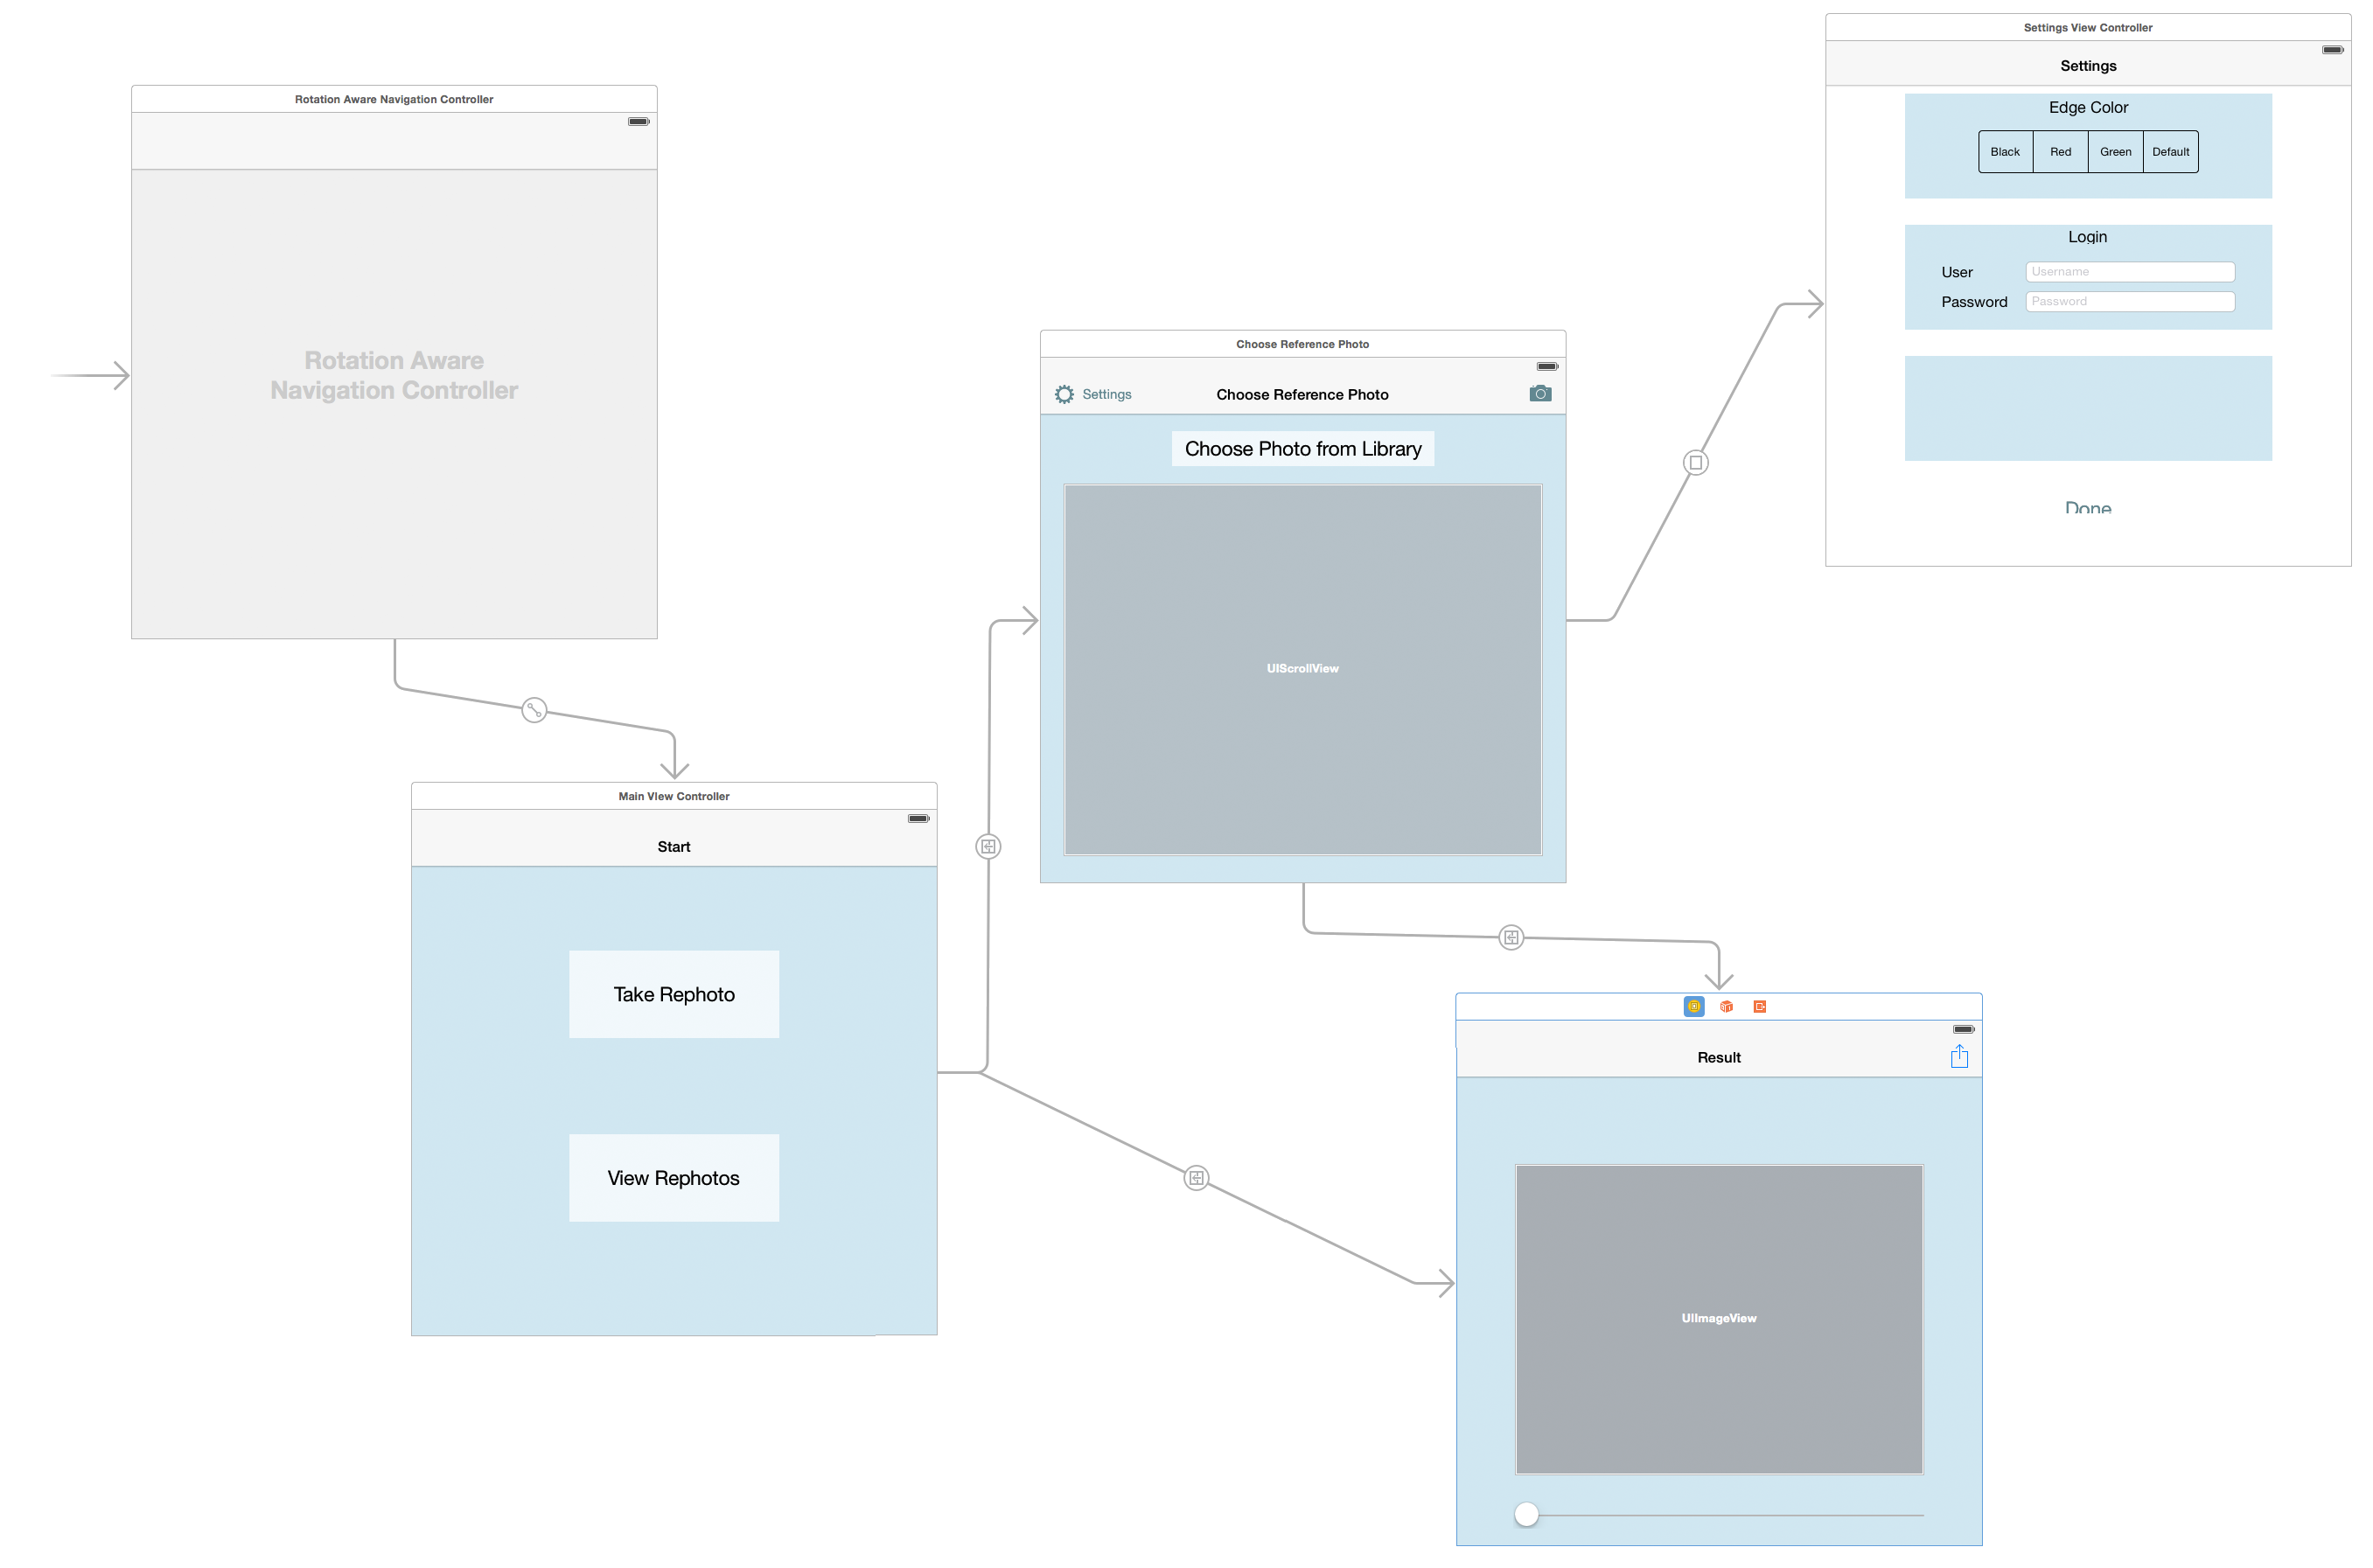
\includegraphics[width=\textwidth]{gfx/storyboard.png}};
   \spy[
      every spy on node/.append style={ultra thick},
      spy connection path={
         \draw[ultra thick] (tikzspyonnode) -- (tikzspyinnode);
      }
   ] on (6.5,-3) in
   node[fill=white,ultra thick] at (6,-10);
\end{tikzpicture}

      \caption[Storyboard example]{The Storyboard of this application. There is
      always a root view controller on whose stack new controllers are pushed or
   popped from, here on the top left. The different view controllers are
connected by segues. The navigation controller on the top left initially has a
Main View Controller pushed on its stack. This one is connected with other
controllers with different actions attached to the two buttons and so forth.
Inside the storyboard, the actual user interface can be created with
drag-and-drop of widgets.}
   \label{fig:storyboard}}
\end{figure}

\FloatBarrier

\subsection{The OpenCV Library}

For all image processing, the Open Source Computer Vision library \citep{opencv} is
used in version 3.0. Originally developed by Intel and then by Willow Garage,
development is led today by itseez\footnote{\url{http://itseez.com/OpenCV/}},
but is strongly community-driven. The library contains many algorithms for image
processing for purposes such as segmentation, geometric transformation, feature
and object detection and 3D reconstruction. It can be natively used from C++,
but Python and Java bindings as well as a deprecated C API exist.  The modules
used in this work are the \texttt{features2d} and \texttt{calib3d} modules for
feature extraction and multiview geometry (pose recovery), respectively.\footnote{Pose recovery
   functions for calibrated images were unavailable prior to version 3.0.
Furthermore, the new version moved all patented feature detection algorithms to a separate
repository.}

\subsection{Mixing Objective-C \& C++}

OpenCV encodes images in its \code{Mat} data type, which is the only C++ type
also used in other (Obj-C) parts of the application.  While it is possible to
mix Objective-C and C++ code, using C++ types in header files forces every
client including them to also be compiled as Objective-C++, which may be
unwanted. For instance, XCode's refactoring tools cannot be used on these
sources. It is thus reasonable to create wrapper classes for all C++ types
encapsulating the access to the data so that the interface is pure Objective-C.
Only the implementation of the wrapper class would need to be compiled as
Objective-C++, no client would be affected. A large amount of boilerplate code would
be required to translate Objective-C messages to the wrapper in C++ calls to the
wrapped object.  It is therefore convenient to encapsulate a C++ type but make
it still accessible to client classes if needed. 

One way of limiting the Objective-C++ to one class is a variant of the
\emph{Pointer-to-Implementation} pattern (PIMPL, also known as \emph{Bridge} in
\citep{gamma1995}). The wrapper class' interface (\autoref{lst:pimpl}) is
specified in pure Objective-C and contains an opaque pointer to a C
\code{struct} representing the wrapped data as a C type, which therefore does not
lead to compatibility issues as all C code is valid Objective-C. For the
original pattern this allows modifying the wrapper hierarchy independently of
the implementation hierarchy (e.g. different implementations could be behind the
pointers for different platforms). The definition of this
pointer-to-implementation type is placed in a second header file
(\autoref{lst:pimpl2}) and is imported only by those clients which actually need
to access the data, not only pass it on. This permits compiling only those
source files as Objective-C++ that must deal with the actual OpenCV \code{Mat}.
In principle it would be possible to create methods in the wrapper class for
all uses of the C++ type throughout the program. However, this would waste the
benefits which e.g. C++ operator overloading yields for readability as all
operations would have to be node with method calls. Since all
image processing is done in C++ anyway, it is more economic to simply provide
access to the wrapped data to those classes that need it.

\lstset{
   language=[Objective]C,
   float,
}

\begin{lstlisting}[
   caption={\code{CVMatWrapper.h}. The wrapper interface contains an opaque pointer to a C
      \code{struct}. including this header does not invalidate
   othewise valid Objective-C code.},
   label={lst:pimpl},
]
struct CVMatWrapperImpl;
@interface CVMatWrapper : NSObject
@property (nonatomic,readwrite) struct CVMatWrapperImpl* impl; ///< Pointer to struct wrapping the matrix
@property (nonatomic,readonly) int rows; ///< Number of rows of the wrapped matrix
@property (nonatomic,readonly) int cols; ///< Number of columns of the wrapped matrix
-(NSArray*)eulerAngles;
-(NSString*)description;
@end
\end{lstlisting}

\begin{lstlisting}[
   caption={\code{CVMatWrapperImpl.h}. The implementation header defines the actually wrapped type.
      Including it will force a client to compile as Objective-C++ since a C++
      type is used. Every class which deals with the data itself can include this
   header in addition to the wrapper one.},
   label={lst:pimpl2},
]
struct CVMatWrapperImpl {
   cv::Mat cvMatrix; ///< The wrapped matrix
};
\end{lstlisting}

\begin{lstlisting}[
   caption={\code{CVMatWrapper.mm}. The wrapper class' implementation must be Objective-C++ and can
   encapsulate all access to the underlying data, if necessary.},
   label={lst:pimpl3},
]
#import "CVMatWrapper.h"
#import "CVMatWrapperImpl.h"

@implementation CVMatWrapper
-(instancetype)init {
   self = [super init];
   if (self) self.impl = new CVMatWrapperImpl; // allocate the struct wrapping the matrix
   return self;
}
-(void)dealloc {
   if (self.impl)
   delete self.impl;
}
-(NSString*)description {
   //...
}
-(NSArray*)eulerAngles {
   // ...
}
-(int)rows {
   return (self.impl->cvMatrix).rows;
}
-(int)cols {
   return (self.impl->cvMatrix).cols;
}
@end
\end{lstlisting}

\section{Application Layout}

This section will walk through the different screens presented to the user and
elaborate on the functions of the associated view controllers. An overview of
the sequence of screens and controllers is shown in \autoref{fig:app_tree}.

\begin{figure}[h]
   {\centering      
      \newcommand{\treenodedist}{1.8}
\begin{tikzpicture}[
      every node/.style={font=\ttfamily,draw=black,thick,anchor=west},
      grow via three points={
         one child at (0.5,-\treenodedist) and
      two children at (0.5,-\treenodedist) and (0.5,-2*\treenodedist)},
      edge from parent path={(\tikzparentnode.south) |- (\tikzchildnode.west)},
      edge from parent/.style={draw,-latex},
   ]
   \node {
      \begin{tabular}{l}
         MainViewController \\
         \rmfamily\small View or make rephotos
      \end{tabular}
   }
   child { node {
         \begin{tabular}{l}
            PhotoChooserController \\
            \rmfamily\small Select original or set settings
         \end{tabular}
      }
      child { node {
            \begin{tabular}{c}
               RephotoManager \\
               \rmfamily\small Retrieve viewpoint
            \end{tabular}
         }
         child { node {
               \begin{tabular}{c}
                  ResultViewController \\
                  \rmfamily\small Review rephoto
               \end{tabular}
            }
            child [missing] {}
         }
      }
      child [missing] {}
      child { node {
            \begin{tabular}{c}
               SettingsViewController \\
               \rmfamily\small Adjust settings
            \end{tabular}
         } 
      }
   }    
   child [missing] {}
   child [missing] {}
   child [missing] {}
   child { node {
         \begin{tabular}{c}
            ELCImagePickerController \\ 
            \rmfamily\small Select rephoto to view
         \end{tabular}
      }
      child { node {
            \begin{tabular}{c}
               ResultViewController \\
               \rmfamily\small Review rephoto
            \end{tabular}
         } 
      }
   };
\end{tikzpicture}

   \caption{Sequence of view controllers. It is always possible to go backwards.}
   \label{fig:app_tree}}
\end{figure}

\FloatBarrier

\newcommand*{\button}[1]{
   \tikzexternaldisable
   \tikz[baseline=-.5ex]{\node[inner sep=1pt,outer sep=0,draw,rounded corners=2pt]{\small\texttt{#1}};}
   \tikzexternalenable
}

\newcommand*{\nofloat}[2]{
   \begin{center}
      \fbox{
         \includegraphics[width=.8\textwidth]{#1}
      }
      \captionof{figure}{#2}
   \end{center}
}

\subsection{MainViewController}

When the app starts up, the user is shown a \code{MainViewController} which
offers a choice whether to make a new rephotograph or view existing ones.
Clicking the \button{Take Rephoto} button will trigger a segue to a
\code{PhotoChooserController}, while tapping \button{View Rephotos} will modally
present an \code{ELCImagePickerController}.

\nofloat{gfx/mainviewcontroller.PNG}{MainViewController view layout}

\subsection{PhotoChooserController}

\setlength\emergencystretch{2em}
This view controller displays a scrollable and pannable view and a button
\button{Choose Photo from Library} to load a reference photograph into it. The
photo is picked from the user's photo album.  Furthermore, the navigation bar
contains a button to access the settings
(\raisebox{-3pt}{
\includegraphics[width=1em]{gfx/settings_icon.png}}, presents a
\code{SettingsViewController}) as well as a button to start the rephotograph
(\raisebox{-1pt}{
\includegraphics[width=1em]{gfx/cam_icon.png}}). The latter
will modally present a \code{UIImagePickerController} which exposes a simple API
to access the device's camera. A
\code{RephotoManager} is attached to it that controls the rephotography. The
\code{RephotoManager} has a delegate property which points to the
\code{PhotoChooserController}. The controller can then be informed when the
rephotograph is done or cancelled.

\nofloat{gfx/photochoosercontroller.PNG}{PhotoChooserController view layout}

When an image is picked, the controller uses the Canny edge detection algorithm
\citep{canny1986} to generate an overlay which will then help the user in
finding the perfect alignment.

\nofloat{gfx/photochoosercontroller_photo.PNG}{PhotoChooserController with loaded image}

\subsection{SettingsViewController}

The \code{SettingsViewController} possesses three panels which allow for
modification of the colour of the edge overlay and insert authentication data for
future use with an envisioned online platform. The third panel is unused in the current
version and could be appropriated for other kinds of preferences such as the default type
of visualisation for the necessary camera motion (see \autoref{ch:outlook}).

\nofloat{gfx/settingsviewcontroller.PNG}{SettingsViewController view layout}

\subsection{RephotoManager}

\hyphenation{Pose-Diff-er-ence-Es-ti-ma-tion-Op-er-at-ion} The two most
important classes are the \code{RephotoManager} and the
\code{PoseDifferenceEstimationOperation}. A \code{RephotoManager} is attached to
a \code{UIImagePickerController} in camera mode and controls the execution of
the rephotograph. An overlay view is added to the camera stream and contains a
shutter button and information labels telling the user what to do next. Tapping
the info button (\raisebox{-2pt}{
\includegraphics[width=1em]{gfx/info.png}})
expands the label to reveal more information. The manager is realised as a state
machine, depicted as a flow chart in \autoref{fig:rephoto_manager}.

\begin{figure}[h]
   {\centering      
      \begin{tikzpicture}[very thick,every node/.append style={text
   centered,font=\small\ttfamily,outer sep=0}]
   \tikzset{>=Latex}
   \node[block] (start) {START};
   \node[block,below=of start] (first frame) {HAS\_FIRST \_FRAME};
   \node[decision,below=of first frame] (can match?) {First and second can be matched?};
   \node[block,below=of can match?] (second frame) {HAS\_SECOND \_FRAME};
   \node[block,below=of second frame] (done) {DONE};

   \path[->] 
   (start) edge node[right=1cm,align=left] {Shutter tapped: \\ First image captured} (first frame) 
   (first frame) edge node[right=1cm,align=left] {Shutter tapped: \\ Second image captured} (can match?)
   (can match?.west) edge[bend left=50] node[left] {No} (start.west)
   (can match?) edge node[left] {Yes} (second frame)
   (second frame) edge[loop left] node[above=2em] {Automatic capture} ()
   (second frame) edge node[right=1cm,align=left] {Shutter tapped: \\ Final image captured} (done)
   ;
\end{tikzpicture}

      \caption{States of the rephoto manager object}
   \label{fig:rephoto_manager}}
\end{figure}

\subsubsection*{\code{START}}

Initially, the user interface presents shutter and cancel buttons in a toolbar
at the bottom and an info indicator on the top left, telling the user the take
the first frame. When the user taps the shutter button, the first frame is
captured and saved.

\subsubsection*{\code{HAS\_FIRST\_FRAME}}

When transitioning to this state, the manager changes the info label accordingly
and displays a check mark for the first frame in the centre of the toolbar.
Furthermore, at this point the precomputed edge overlay is presented so that
taking the second frame which should be reasonably close to the original
viewpoint is possible.

\subsubsection*{\code{HAS\_SECOND\_FRAME}}

Once the second frame is captured, the second check mark is shown, the info
label changes again and the preprocessing step is attempted. A
\code{PoseDifferenceEstimationOperation} is started with the first and reference
frames to obtain $T_{ref,first}$ and $R_{ref,first}$ to be used in
\eqref{eq:necessary_trans}. A second operation is run for the reference scale
computation by use of first and second frames. Relative translation, rotation
and goal scale are saved.

Should one of the computations fail, the user interface resets to the initial
state except for an error label at the bottom centre informing the user that the
matching failed, underpinned by a red box. Otherwise a timer is initiated that
will take pictures at a certain interval which should accord with the hardware
running the program. For the tested device, it is set to one second, although
somewhat higher frame rates are possible. For each frame captured like this, a
\code{PoseDifferenceEstimationOperation} (see below) is started. The captured
frame and the first frame are processed and their relative pose computed. With
the information computed during preprocessing, the necessary translation is
inferred with \eqref{eq:necessary_trans}.

Meanwhile, a panel at the bottom centre is revealed which visualises this
necessary motion of the camera. For this, several means are possible and
discussed in \autoref{subsec:alternative_visualisation}.
\citet{bae2010} found that an arrow visualisation for the translation in the
XY-plane and Z-direction is most effective so this approach has been chosen
here. Two camera pictograms are shown, one back view and one top view. There is
one arrow positioned on each so that the translation in the XY-plane and
Z-direction are independently visualised.

\nofloat{gfx/rephoto_manager.PNG}{RephotoManager after second frame was captured}

\subsubsection*{\code{DONE}}

Once the final image is taken, the controller informs its delegate that the
rephotograph has finished and passes the final capture. The delegate---in this
case the \code{PhotoChooserController}---can then put together an
\code{ImageData} object to present the rephoto to the user.

\subsection{ResultViewController}


This controller must be passed a completed rephotograph in an \code{ImageData}
object and displays the new image over the original.  With a slider, the new
image is horizontally clipped to some percentage of its width and can thus be
dynamically unrolled over the original. Depending on a flag in the
\code{ImageData} object, the rephoto passed to the controller will be saved. For
this, the app makes use of the \code{sqlite} library. The \code{DBManager} class
manages communication with a lightweight SQL database. Since all photos are part
of the user's photo library---there is no way to save assets locally for an
application---they are saved as a tuple of two \code{NSURL}s. Both the built-in
\code{UIImagePickerController} and the \code{ELCImagePickerController} return
the URL of a selected image so it can be used to map a rephoto on its original
or vice versa when it should be displayed.

\nofloat{gfx/resultviewcontroller.PNG}{ResultViewController view layout}

\begin{wrapfigure}{r}{.25\textwidth}
   \includegraphics[width=.2\textwidth]{gfx/image_data.pdf}
\end{wrapfigure}
On the top right, a share button (\raisebox{-3pt}{
\includegraphics[width=.8em]{gfx/share.png}})
lets the user upload a rephoto to an experimental test server for display, but the
functionality is only rudimentary and requires the server to be running with a known IP address.

\subsection{ELCImagePickerController}

For the task of reviewing rephotographs, the \code{ELCImagePickerController} is
used. Contrarily to the built-in \code{UIImagePickerController}, this
reimplementation by \citet{nutting2013} allows to inspect a specific asset, like
a photo album instead of all assets there are. In the album display, the user is
shown the new photographs of each rephoto and upon selection is presented a
\code{ResultViewController} with the rephotograph.


\section{Implementation}

This section will survey the more important pieces of the software and elaborate
on the particular challenges addressed by them. The implementation of the
relative pose estimation is described in detail.

\subsection{User Interface}

For the user interface several custom views classes are implemented.
\begin{enumerate}
   \item \code{ArrowView} A view which is backed by an \code{ArrowLayer} and
      allows displaying it as \code{CALayer}s cannot be shown without a
      wrapping \code{UIView}.
   \item \code{ArrowLayer} A \code{CALayer} subclass which can display a
      parametrisable arrow shape whose parameters can be seamlessly animated.
      \code{CALayers} are the backbone of all \code{UIView} objects.
   \item \code{ImageScrollView} A \code{ScrollView} subclass which allows
      displaying a zoomable and pannable image while also preserving the visible
      portion when the user interface orientation changes.
   \item \code{CircleView} A simple view purely for drawing a circle parametrised
      with colour and line width.
   \item \code{MaskableUIImageView} An \code{UIImageView} which allows the
      image to be clipped to some percentage of its width. This is used to
      display a before-after comparison of the original and repeat photographs.
\end{enumerate}

Furthermore, two view hierarchies and the storyboard belong to this module.  If
a custom view must exhibit some particular behaviour which necessitates custom
methods, creating classes is appropriate. For interface elements which contain a
larger hierarchy of nested views without exposing any particular behaviour
besides what the contained views can do,
specifying them in a visual manner is less involved. Such view hierarchies can
be built visually as \code{XIB} files in an XML format. The
\code{CameraOverlay} overlayed on the current camera picture is created like
this, as well as the launch screen shown when starting the app.


\subsection{Image Processing}

\hyphenation{com-pute-Po-se-Diff-er-ence-Be-tween-Cam-er-a:-sec-ond-Cam-er-a:-cal-i-bra-tion-File:-sca-le:}
% dirty hack

The bulk of the work is done inside the utility class' \code{ImageUtils} static
methods. To compute the pose difference between two frames, clients can call the
public method
\code{+[computePoseDifferenceBetweenCamera:secondCamera:calibrationFile:scale:]}.
The two images must be passed, as well as the path to a calibration file in
OpenCV's \code{FileStorage} format. A scale parameter can be used to speed up
the computation by downsampling the images.  The scale is set to $0.33$,
compromising between speed and matching robustness. This number takes into
account that compared to the computations performed on a computer (see
\autoref{ch:evaluation}) some detail is lost during conversion between iOS's
\code{UIImage} format and OpenCV's \code{Mat} type.

Internally, the method converts the images, uses OpenCV image processing
functions to compute the pose difference, and the average distance of the matched
features to the first camera. The client is returned an \code{NSDictionary}
containing the rotation, translation, average point distance, and---should the
computation fail---an error code in which case all other values are invalid.

The method first runs \texttt{AKAZE} on both images, the parameters used are
shown in \autoref{tab:akaze_params}.  Computation is aborted if one of the
images yields fewer than $100$ keypoints.  Matches are found by brute force with
a ratio test as suggested by \citet{lowe2004}. Let $d(x,y)$ denote the distance
(here the $L_2$-norm) of descriptors $x$ and $y$. For all descriptors $x$ in the
first image, the two best matching descriptors $y_1$ and $y_2$ in the other
image are found. If
\begin{equation*}
   \frac{d(x,y_1)}{d(x,y_2)} < \rho
\end{equation*}
then the pair $(x,y_1)$ is chosen as a match. Lowe suggests $\rho=0.8$, the app
uses a stricter ratio of $\rho=0.7$. This test will filter unstable matches
between e.g. repeating patterns in an image (windows, wall structure etc.) as
for such a point the corresponding point is very ambiguous and its best matches
will be similar in distance.

The function then removes the image distortion (see \autoref{subsec:intrinsics})
on the sparse set of keypoints instead of the whole image for
efficiency.\footnote{Since undistortion requires resampling of the image, it is
   better to find features beforehand as some information may be lost by
interpolation.} On the correspondences, RANSAC and the five-point algorithm are
used to find the best-fitting essential matrix. The confidence
threshold is set to $0.999$, a point is considered an outlier if its distance
to its epipolar line exceeds $3$ pixels.  

Once $E$ is fixed, the optimal triangulation method (see \citet[ch.  12.5.2]{h&z2004})
is used to correct the corresponding points. Since one assumes
the computed essential matrix is correct, the information can be used to
refine the position of corresponding points. This should make pose recovery
with $E$ and the points more accurate.

The essential matrix is then decomposed into $R$ and $T$. A sanity check for a valid rotation
matrix is performed by checking that $|\det R|\approx 1$.\footnote{A rotation
matrix is orthogonal and orthogonal matrices' determinants are $\pm 1$}

\rowcolors{2}{gray!5}{white} % alternating colours
\begin{table}
   \begin{center}
      \begin{tabular}{>{\ttfamily}ll}
         \rowcolor{white}
         \toprule
         \rmfamily Parameter     & Value \\
         \midrule
         nOctaves                & $4$ \\
         threshold               & 0.001 \\
         nOctaveLayers/sublevels & $4$ \\
         descriptor\_size        & $486$
         bits\tablefootnote{\texttt{AKAZEFeatures.cpp line $720$}, commit \texttt{09b9b0f}} \\
         descriptor\_channels    & $3$ \\
         \bottomrule
      \end{tabular}
      \caption[Parameters for AKAZE]{Parameters used for AKAZE (number of octaves, detector response
      threshold, levels per octave, size of the descriptor and the number of
   channels, see \autoref{subsec:sift_akaze})}
      \label{tab:akaze_params}
   \end{center}
\end{table}

\rowcolors{2}{gray!5}{white} % alternating colours
\begin{table}
   \begin{center}
      \begin{tabular}{>{\ttfamily}ll}
         \rowcolor{white}
         \toprule
         \rmfamily Parameter     & Value \\
         \midrule
         nOctaveLayers/Sublevels & $3$ \\
         contrastThreshold       & 0.04 \\
         edgeThreshold           & $10$ \\
         sigma                   & $1.6$ \\
         \bottomrule
      \end{tabular}
      \caption[Parameters used for SIFT]{Parameters used for SIFT (number of octaves, number of sublevels
      per octave, detector response threshold, edge threshold for filtering
   edges, standard deviation of the Gaussian for the initial image)}
      \label{tab:sift_params}
   \end{center}
\end{table}

\subsection{Categories}

Code reuse in Objective-C can be accomplished by inheritance as in other
object-oriented languages. But when only one piece of behaviour is to be
added, not overridden\footnote{The behaviour is undefined when a Category method
has the same signature as one of the class \citep{customizing}}, the
lightweight Category concept is often employed instead. A Category on a class adds methods
or properties to that class. The header file declaring the category can be
included by all clients that wish to make use of the modified or added
behaviour, and left out by all others. This way, no unnecessarily large class
hierarchy is created.

In this application, categories are used for different purposes. They are
summarised in \autoref{tab:categories}.

\begin{table}
   \begin{tabularx}{\linewidth}{>{\ttfamily}p{4cm}X}
      \toprule
      \rowcolor{white}
      {\rmfamily Category Name}           & Function \\
      \midrule
      NSMutableURLRequest (RephotoUpload) & Adds method to post a rephoto to an
      experimental server via HTTP \\
      ALAssetsLibrary (CustomPhotoAlbum)  & Adds method to add an image to a
      specific album, not possible per default. Used to save rephotos to the
      \code{Rephotos} album \\
      NSUserDefaults (UIColor)            & By default, only some types can be
      persistently saved in the user defaults. Adds method to save colours. Used
      to remember the user's edge colour.\\
      CALayer (UIColor)                   & Properties for view objects can be
      set in Interface Builder, but only if they are of object type. To set a
      view's backing layer's border colour outside of the code, a colour
      property of object type is defined, mapped to the C type \code{CGColor}
      used by \code{CALayer}. \\
      UIBezierPath (Arrow)                & Adds a method to generate an arrow
      shape with a bézier curve. Used for displaying user guidance. \\
      UIImage (Zoom)                      & Adds a method to crop an image to a
      rectangle centred on the image centre, effectively zooming in. Used to
      allow the user to zoom the camera image. \\
      UIScrollView (Center)               & Adds methods to centre the content
      and zoom to a particular size. Used for display of the original image. \\
      UIColor (CustomColors)              & Contrarily to Android, iOS possesses
      no Resources framework, so this Category declares some commonly used
      colours for the user interface \\
      UIView (Effects)                    & Adds some animation methods to all
      views to avoid repeating boilerplate code. \\
      \bottomrule
   \end{tabularx}
   \caption{Summary of categories}
   \label{tab:categories}
\end{table}

\FloatBarrier

\subsection{Computation Of Necessary Translation}

\begin{wrapfigure}{l}{.35\textwidth}
   \includegraphics[width=.35\textwidth]{gfx/posediffop.pdf}
\end{wrapfigure}
The computation of the necessary translation is implemented by the
\code{PoseDifferenceEstimationOperation} class and was conceived to allow
parallelisation.

iOS supports different APIs for concurrency. Besides manual thread creation,
Grand Central Dispatch allows to easily dispatch blocks (function objects) to
different kinds of dispatch queues. The runtime automatically removes blocks
from the queues for execution. Dispatch queues can be serial or concurrent and both
synchronous and asynchronous dispatch is possible as well as synchronisation,
but the API is not object-oriented and some useful features are unavailable. It
is not possible to specify how many blocks should be executed in parallel or to
cancel tasks after submission. Since the application should make optimal use of
the hardware due to high computational demand while not queueing up many tasks
or tasks which are obsolete, such functionality is desirable.

Operation queues---internally implemented with
GCD\footnote{\citep{nsopgcd}}---sacrifice some efficiency, but expose a more
high-level object-oriented interface in which \code{NSOperation} objects are
submitted to \code{NSOperationQueue}s and their
\code{maxConcurrentOperationCount} property limits the maximum number of
concurrent operations. The application sets this limit to $3$ for an iPad
(assuming $3$ cores like an iPad Air 2) and $2$ for iPhones, as the current
devices possess two cores. Since there is no concurrent modification of data and
tasks are started in slow intervals, explicit synchronisation is not needed.

A \code{PoseDifferenceEstimationOperation} is created with two images (one of
which will always be the first frame), a scale parameter for downsampling, and
computed values for the relative pose between first and reference frames and the
goal scale. Furthermore, a completion block is passed which can accept three \texttt{float}
parameters---one for the direction in the XY-plane, one for the ratio between
reference and current world scale, and one for the magnitude of translation along
the optical axis. The intended purpose of this block is to drive some kind of
visualisation. The operation then computes the relative pose and the necessary
translation as in \eqref{eq:necessary_trans}. 

If $\sub{T}{current,ref} = (x,y,z)$\footnote{One should note that this
   calculation depends on the coordinate system. In OpenCV, the origin is at the
   top left corner of an image, the positive $x$-axis is the image width, the
   positive $y$-axis the image height and points downward. In a more canonical
representation, the $y$-value thus may be flipped}, then the vector direction
in the XY-plane is given by 
\begin{equation*}
   \alpha = \atan2{(y,x)}.
\end{equation*}
Let $d_0$ be the average distance of scene points to the first frame's camera,
computed with the second frame, and $d_i$ the same with the current frame. The
ratio of scales $r=\frac{d_i}{d_0}$ is used to scale the translation vector. $d_i$
increases with decreasing distance to the first frame (see \autoref{fig:scale}),
which in turn (usually) means it should decrease when approaching the target,
since when done right, motion away from the first frame is motion towards the
original viewpoint.

The completion block is called with $z$, $\alpha$ and $r$.

\section{Hardware}

The application has been developed on an iPad Air 2. This model features an
A8X processor with three cores and $1.5$GHz per core.\footnote{The number is not
official and based on empirical tests \citep{a8x}} The number of concurrently
running \code{PoseDifferenceEstimationOperation}s is thus set to three which
enables frequent updates of the visualisation. Images with $1077\times 807$
(full resolution with a $0.33$ scale factor) take roughly $0.7$ seconds to
process, so that updates can be delivered more than once per second. The
concurrent operation count is set to two for iPhones owing to their smaller
processing power and number of CPU cores.
